\documentclass[../main.tex]{subfiles}

\begin{document}
	\section{Resultate}
	
	\subsection{Frontend}
	
	Als Frontend haben wir 3 Menüpunkte ausgewählt, welche die Hauptfaktoren unserer Schnittstelle aufzeigen. \\
	Der erste Punkt ist die Übersicht. Hier werden die aktuellen Systeme mit Tanks und die Hauptsensorendaten aufgeführt. \\
	Für alle Sensorendaten gibt es einen Editierbutton, mit welchem die Daten geändert werden können.\\
	Unterhalb jedes Systems gibt es die Details Option. Über diesen gelangt man zu den detaillierten Infos jedes Tanks des oben genannten Systems in der unteren Abbildung Angular Frontend. \\ \\
	Das tabellarische Layout ist an das Design des SC1000 angelehnt, damit mit einer gewohnten Umgebung weitergearbeitet werden kann. 
	\begin{figure}[H]
		\centering
		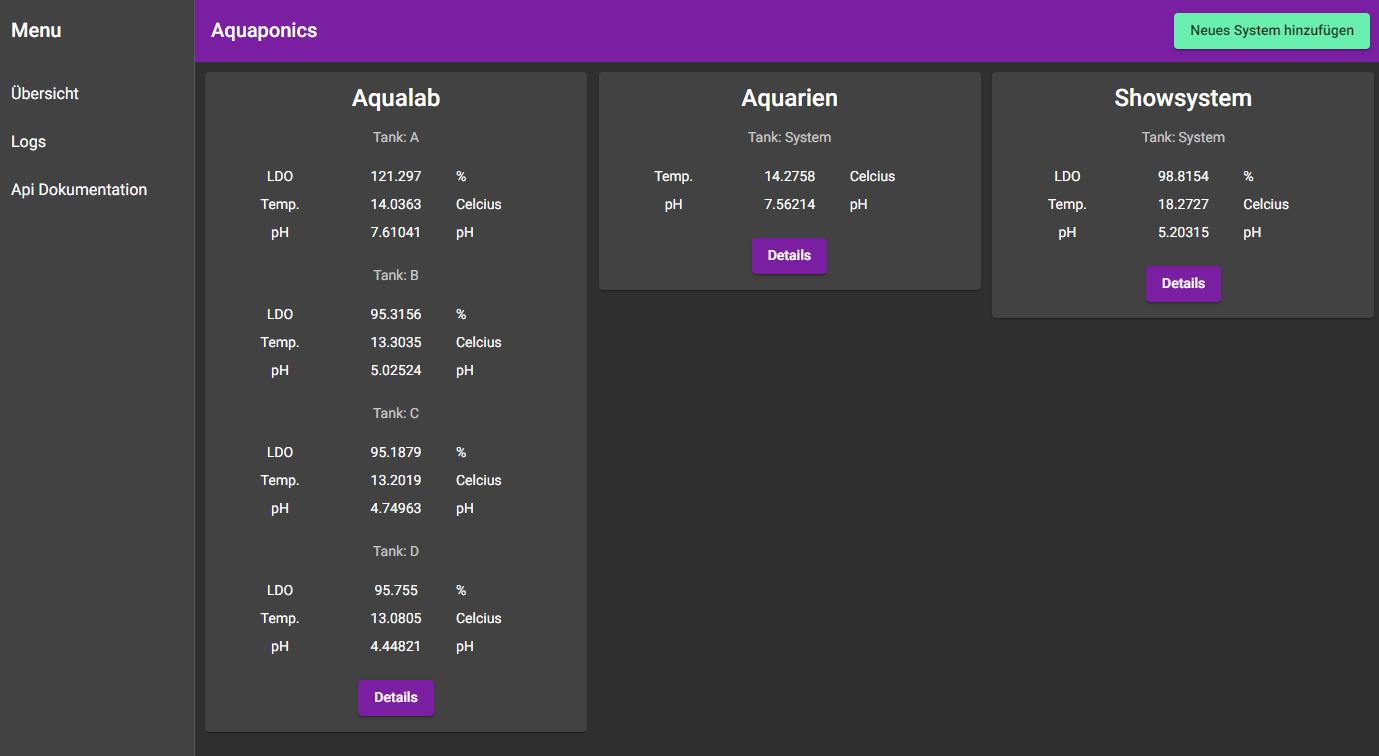
\includegraphics[scale=0.4]{Frontend_Dashboard}
		\caption{Übersicht}
		\label{fig:Frontend_Dashboard}
	\end{figure}
	\par
	\noindent
	Der zweite Punkt ist Logs. Hier sind alle Daten über einen älteren Zeitraum archiviert worden. Die Daten sind wichtig um zu vergleichen, wie sich Veränderungen über eine längere Zeit gebildet haben. Die Logdaten sind eins zu eins aus der Datenbank geladen und werden dort immer aktualisiert. Hier sind auch Sensorennummer und Zeitstempel enthalten damit keine Verwirrung auftritt.
	
	\begin{figure}[H]
		\centering
		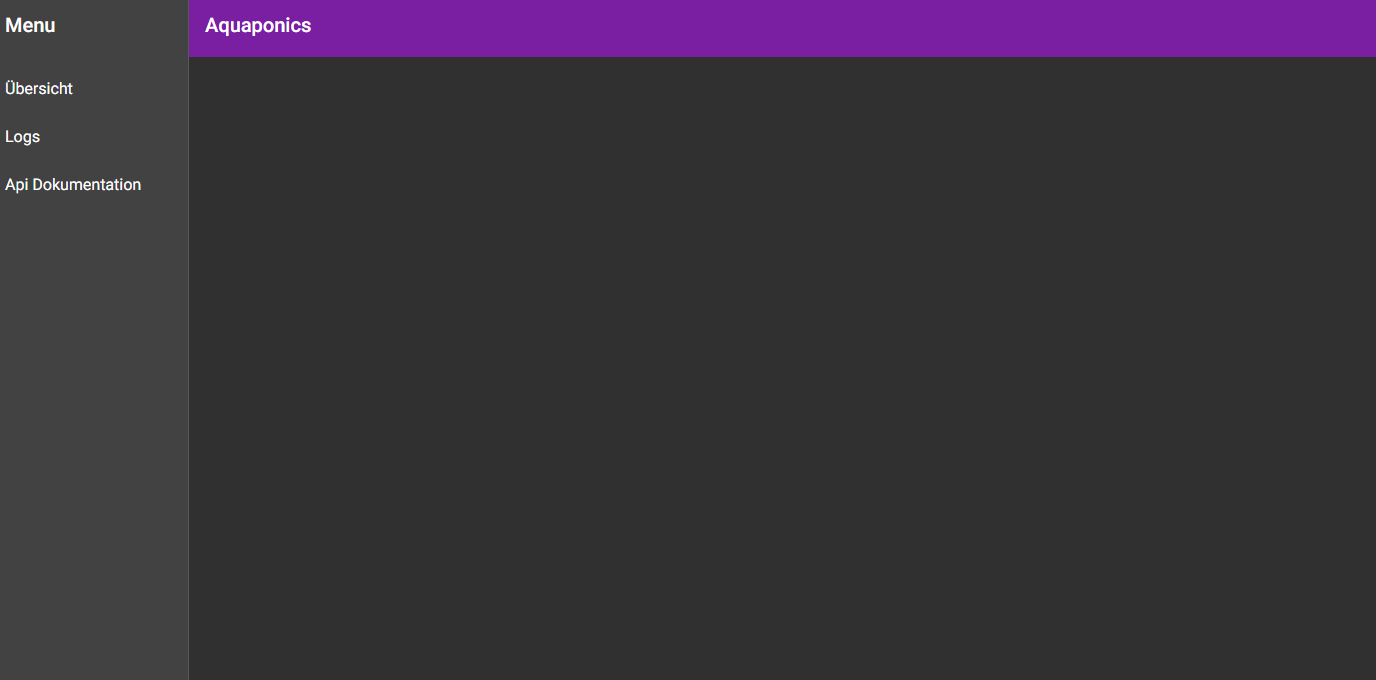
\includegraphics[scale=0.4]{Frontend_Logs}
		\caption{Logs}
		\label{fig:Frontend_Logs}
	\end{figure}
	\par
	\noindent
	Als letzter Menüpunkt wird noch auf die API Dokumentation verwiesen, welche sich auf die Swagger UI bezieht. Dort sieht man alle Eigenschaften und andere Wissenswerte Details über die Schnittstelle für zukünftige Entwicklungen.\par 
	\begin{figure}[H]
		\centering
		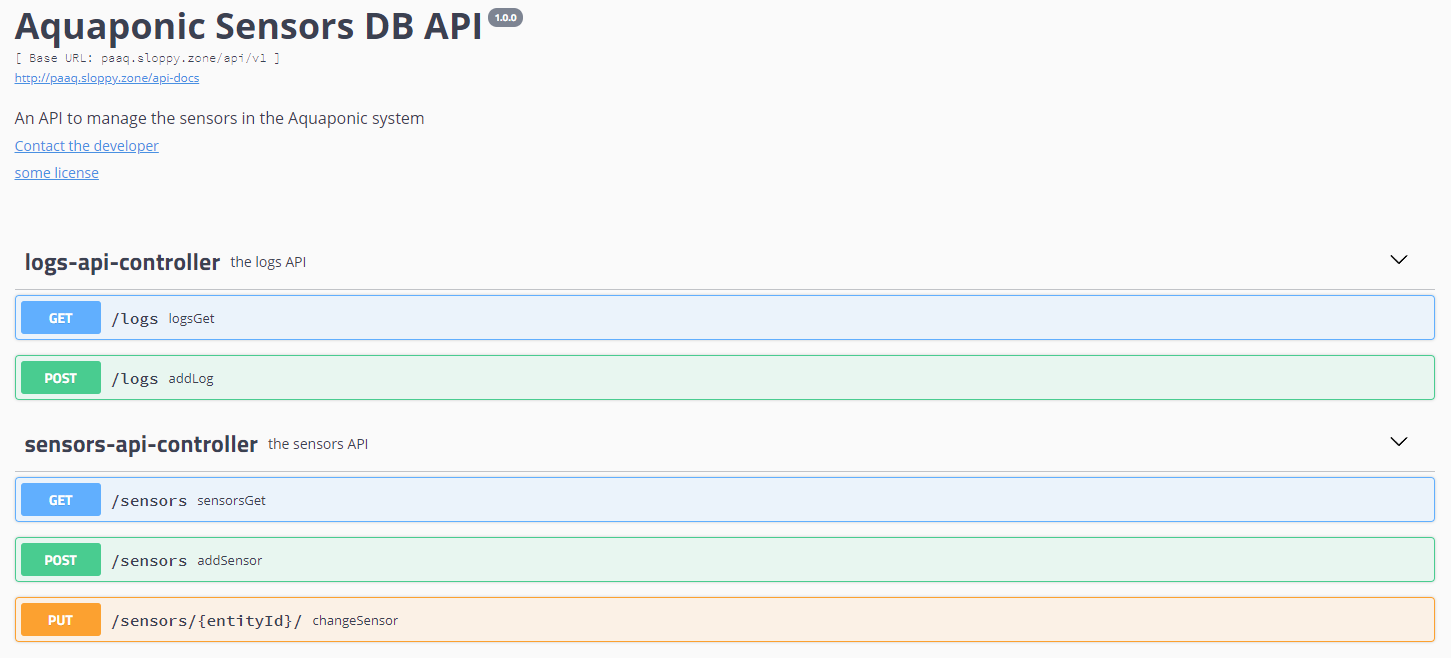
\includegraphics[scale=0.4]{../images/API_Documentation}
		\caption{API Dokumentation}
		\label{fig:API_Documentation}
	\end{figure}
	\noindent
	Wie auf der Abbildung ersichtlich ist, werden verschiedene API Aufrufe über das Aufrufen des Dashboards oder das Klicken auf den Editierbutton in den Sensorendaten gesteuert. 
	\\
	Somit wird das Arbeiten mit den Sensorendaten um ein Vielfaches erleichtert.
\end{document}